\newcommand*{\antikt}{anti-$\kappa_{t}$\xspace}
\newcommand*{\etmiss}{$E^{\text{miss}}_{\text{T}}$\xspace}
\newcommand*{\tauhadvis}{$\tau_{\text{had-vis}}$\xspace}
\newcommand*{\tauhad}{$\tau_{\text{had}}$\xspace}
\newcommand*{\ttbar}{$\bar{t}t$\xspace}

Once the High Level Trigger accepts an event, the collision data are recorded and processed offline to reconstruct the particles emerging from the proton–proton collision. 
Signals in the ID, calorimeters and MS are combined by dedicated algorithms to form the physics objects used throughout this thesis: charged-particle tracks and collision vertices, muons, electrons and photons, jets, including heavy-flavor tagging, hadronically decaying $\tau$-leptons, and missing transverse momentum. Figure~\ref{fig:reco} shows a schematic description of different fundamental particles interacting with the \acrshort{ATLAS} detector. 
To accommodate diverse analysis requirements, each reconstruction algorithm offers multiple working points (WPs), trading off identification efficiency against background rejection. This chapter describes the algorithms used to reconstruct the different physics objects, with emphasis on those most relevant to the measurements presented in this thesis, whereas electrons are discussed more extensively in Chapter~\ref{chap:electrons}.

\begin{figure}[h]
  \centering
  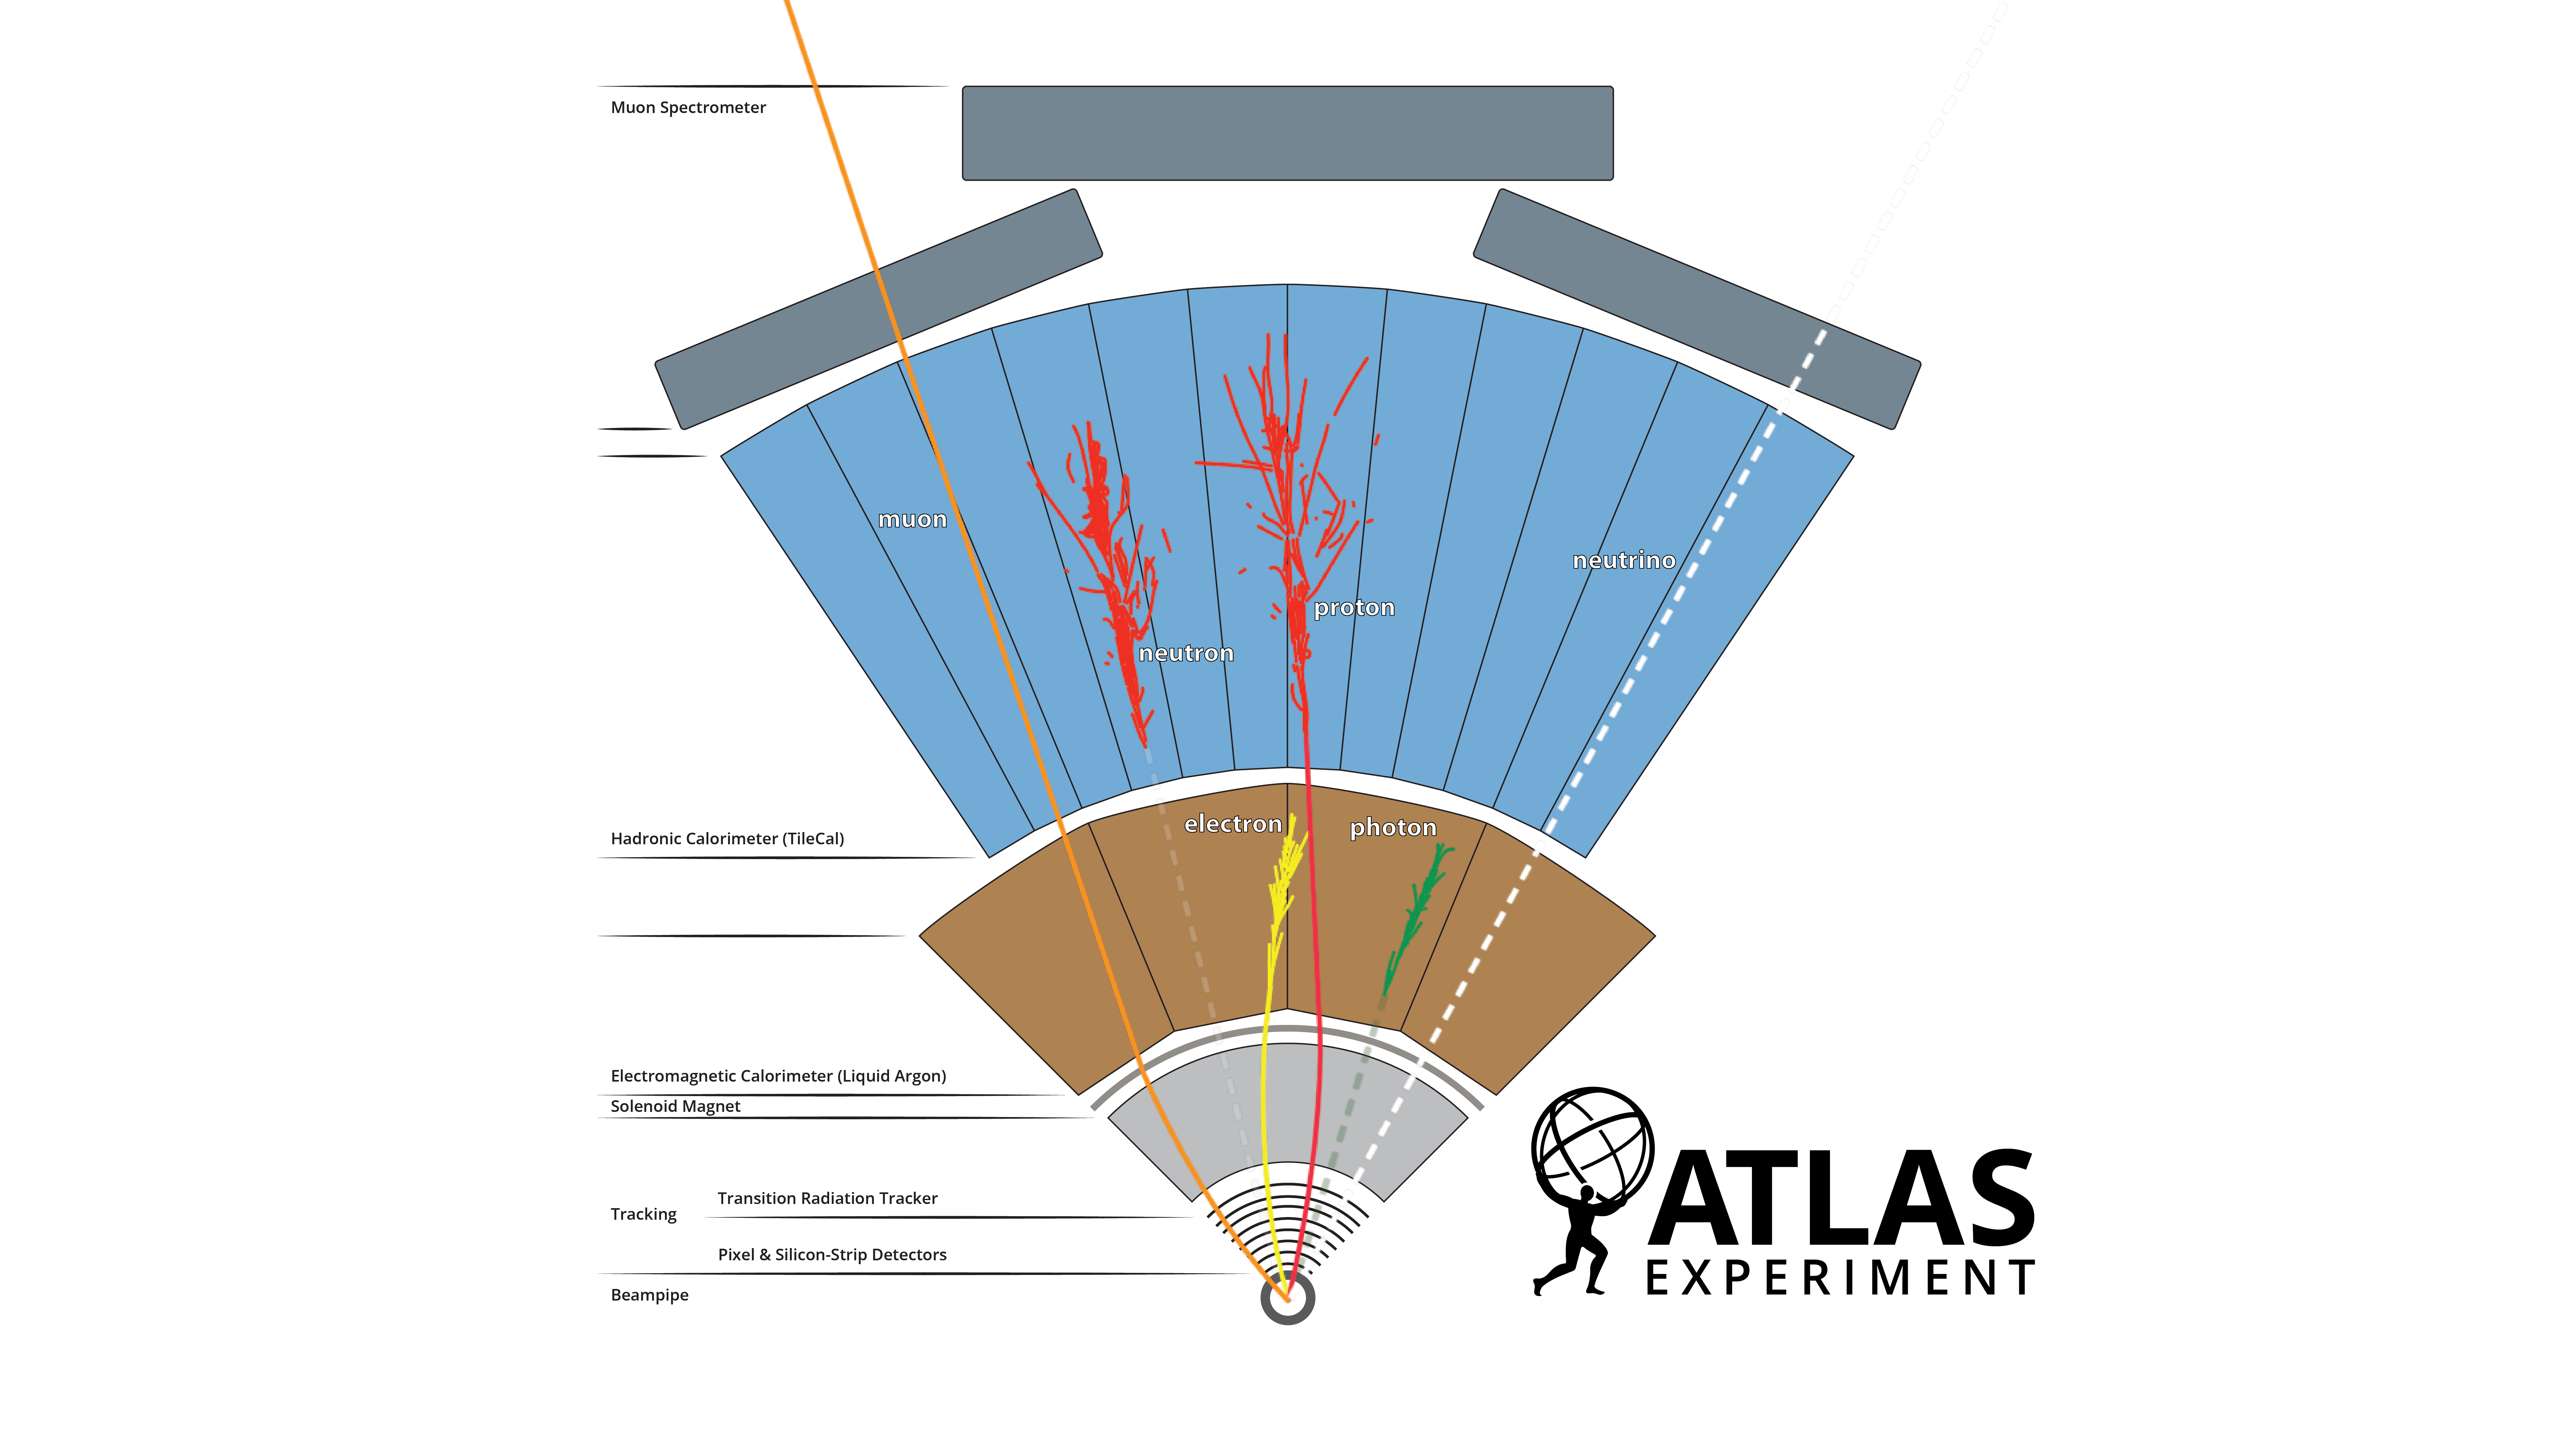
\includegraphics[width=0.9\textwidth]{images/atlas_particles.png}
  \caption{Schematic representation in the $x-y$ plane of fundamental particles interacting with the different ATLAS sub-systems~\cite{Bianchi:2837191}.}
  \label{fig:reco}
 \end{figure}

\section{Tracks and vertices}
\label{sec:tracks}

As mentioned before, tracks, vertices and calorimeter energy clusters, as well as matching requirements among themselves, are the essential inputs to the reconstruction and identification of physics objects which are going to be discussed in this chapter.

The first step in the reconstruction of an event is the identification of the trajectories defined by charged particles in the ID, which are called tracks.
Charged particles traversing the ID leave spatially precise hits in the Pixel and SCT layers, followed by the TRT. Under the solenoidal 2~T magnetic field, their paths bend into helices, with curvature inversely related to transverse momentum. 
Each reconstructed track is described by five parameters: transverse momentum \pt, polar angle \(\theta\), azimuth angle \(\phi\), the impact parameter in the transverse plane with respect to the interation point \(d_0\), and longitudinal impact parameter, in the longitudinal plane \(z_0\). Figure~\ref{fig:tracks} shows a representation of those parameters.

\begin{figure}[htbp]
  \centering
  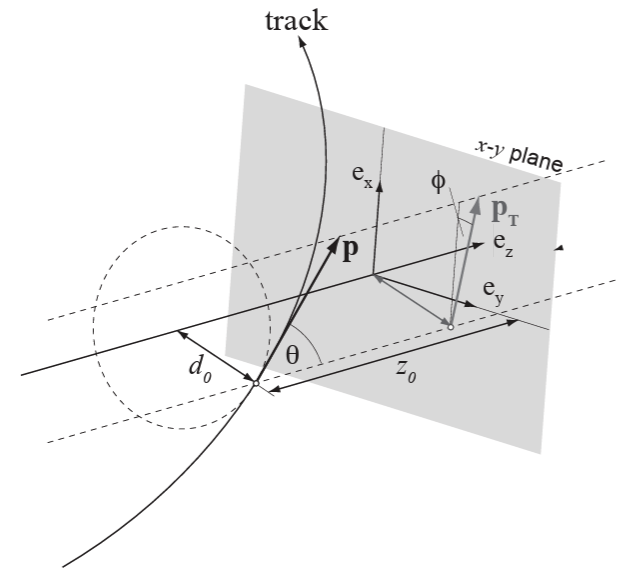
\includegraphics[width=0.6\textwidth]{images/tracks.png}
  \caption{Schematic representation of a track and the different parameters that are used to describe it in ATLAS. The $e_z$ direction follows the beam line\cite{Bianchi:2837191}.}
  \label{fig:tracks}
 \end{figure}

The reconstruction proceeds in several stages~\cite{tracks}. First, nearby hits or sensor measurements above a threshold are clustered and triplets of clusters form track seeds. Next, a combinatorial Kalman filter~\cite{kalman} extends each seed outward, adding compatible clusters layer by layer and updating the track parameters at each step (i.e. the momentum or its position). Multiple overlapping candidates are pruned by an ambiguity solver, which scores each track using fit \(\chi^2\), \pt, the number of associated clusters, and the count of “holes” (expected but missing hits), to favor well–measured and high-\pt trajectories.

Finally, surviving candidates undergo a global fit, incorporating all valid clusters to refine the five helicoidal parameters. The chosen tracks are required to have at least 7 clusters between the Pixel and the SCT detectors, less than 2 holes in the Pixel and a maximum of 2 holes in the SCT sub-detector, a $p_{\text{T}} > 500$~MeV and a $|\eta|>2.5$. In addition, the track is required to satisfy $|d_0|<2$~mm and $|z_0\sin\theta|<3$~mm, and then it is retained for downstream object reconstruction.

Subsequently, the tracks are used to reconstruct vertices, which correspond to the locations where particle interactions occur. Vertices are identified by extrapolating tracks backward to their point of closest approach. Vertices occurring near the proton–proton interaction region are of key interest. The primary vertex of an event is defined as the point where the hard-scattering interaction occurs, while all other reconstructed vertices are treated as pile-up or secondary vertices, which are also crucial for 
flavour tagging and identifying other displaced objects. A detailed description of primary-vertex reconstruction in ATLAS can be found in Refs.~\cite{vertex_run1,vertex_run2,vertex_run3}.

Generally, vertex reconstruction proceeds in two phases: finding and fitting. First, vertex finding groups tracks into vertex candidates. An initial seed position is chosen, and then an iterative fit adjusts both the vertex position and individual track weights, which quantify how well a track originates from that vertex. Tracks whose weights fall below a threshold at the final iteration are excluded and reserved for forming additional vertices. This cycle is repeated on the remaining unassigned tracks until no further vertices emerge. 
Next, vertex fitting refines the three-dimensional location of each candidate using its assigned tracks. The event’s primary vertex is defined here as the one whose tracks have the largest $\sum p^2_{\text{T}}$, although alternative primary-vertex definitions exist.

\section{Energy clusters}
\label{sec:clusters}

Particles leave energy deposits in individual cells of ATLAS calorimeters, which are clustered together forming three-dimensional topological cell clusters, called topoclusters~\cite{topo}.

Topoclusters are constructed by first identifying seed cells whose measured signal exceeds the expected electronics noise by a significant amount. From each seed, adjacent cells are added iteratively whenever their signal-to-noise ratio passes a predefined threshold, and this expansion ceases once no further cells meet that criterion. Cells with low significance are excluded, naturally filtering out noise. Because hadronic showers spread more broadly than electromagnetic ones, a single topocluster may capture an entire shower, only part of it, or even combine energy deposits from multiple particles. 

Since the ATLAS calorimeters are non-compensating, which means that their response to hadrons is lower than to electrons or photons of the same energy, all signals are initially recorded on the electromagnetic energy scale. To account for the differing responses and energy losses in inactive materials, topoclusters undergo dedicated calibrations. After calibration, each cluster can be treated as a massless pseudo-particle, described uniquely by its calibrated energy and position in the $\eta - \phi$ space. 

Actually, during Run~2, the reconstruction of physics objects further incorporated the concept of superclusters, obtained by dynamically grouping together several adjacent topoclusters in the electromagnetic calorimeter. This approach improved the ability to capture energy lost through bremsstrahlung photon emissions, and became a key element in particular for electron reconstruction. A detailed discussion of superclusters, together with an illustrative diagram, is provided later in Chapter~\ref{chap:electrons}.

\section{Muons}
\label{sec:muons}

Muons are reconstructed and identified using combined information from the ID and the MS. These minimum-ionizing particles with long penetration length through the calorimeters leave very small energy deposits in the subdetectors.
\subsection*{Reconstruction} 
Track candidates are first found independently in the ID and in the MS. In the ID, the tracks are reconstructed as explained in Section~\ref{sec:tracks}.

In the MS, track fragments are formed by combining hits that lie close together along the expected trajectory of a muon and that are consistent with having originated from the IP~\cite{muon_reco_run2}. 
In order to create seeds, segments from the middle station of the MS are first used, and these seeds are then extended into the inner and outer detector layers. A track candidate requires at least two such segments, and a given segment may contribute to multiple candidates. Ambiguities are resolved and the candidate is accepted or rejected by performing a $\chi^2$-fit to the hits associated with each track candidate, together with additional track quality requirements.

Once both trajectories are reconstructed in ID and MS, various muon reconstruction categories are defined based on the detector information they exploit. “Combined” muons result from a joint fit of ID and MS tracks, typically using an outside-in strategy that projects MS tracks back into the ID; an inside-out approach, seeding from the ID and extending into the MS, is also employed. “Extrapolated” muons rely uniquely on MS tracks extrapolated to the beamline, ensuring compatibility with the primary vertex, and extend coverage into the forward region $2.5 < |\eta| < 2.7$
beyond the ID acceptance. “Segment-tagged” muons begin with an ID track that is matched to at least one precision chamber segment in the MS, recovering lower-energy muons that traverse only a single spectrometer layer. Finally, “calorimeter-tagged” muons are identified by isolated, minimum-ionizing energy deposits in the calorimeter aligned with an ID track, filling in gaps where MS coverage is incomplete.

\subsection*{Identification} 

On top of reconstruction, the muon identification in ATLAS applies additional selection criteria to the reconstructed muons in order to reduce contribution from background sources like charged hadron decays, in-flight decays, etc.
Seeking for a balance between identification efficiency and background rejection, different working points are defined encapsulationg these selection requirements. The main ones are Loose, Medium and Tight WPs, plus two additional ones devoted to low-$p_{\text{T}}$ and high-$p_{\text{T}}$ muons.

The Loose WP accepts all reconstructed muon types with minimal kinematic cuts (e.g.\ $p_{\text{T}}>4$~GeV), achieving maximal efficiency at the cost of higher fake rates, particularly in the reduced-coverage region $|\eta|<0.1$. The Medium WP restricts to Combined and Inside–Out muons within $|\eta|<2.47$, requires at least three precision-chamber hits spanning two muon-spectrometer layers (one layer suffices for $|\eta|<0.1$), and imposes a compatibility cut on the charge-over-momentum difference between the Inner Detector and Muon Spectrometer measurements of less than seven standard deviations. Finally, the Tight WP further tightens these requirements by demanding a three-hit segment in two distinct spectrometer stations and stronger cuts on the $q/p$ significance and inter-subdetector momentum consistency, all optimized in $(p_{\text{T}},\eta)$ bins to suppress residual backgrounds.

In simulated \ttbar and $Z\to\mu\mu$ samples, the Medium WP achieves prompt-muon efficiencies up to 97$\%$~\cite{muon_reco_run2}, while retaining background muons (e.g.\ from hadron decays) at the per-mille level. Figure~\ref{fig:muon_eff} shows the muon reconstruction and identification efficiencies measured for the three main WPs.

\begin{figure}[h]
  \centering
  \subfloat[]{
      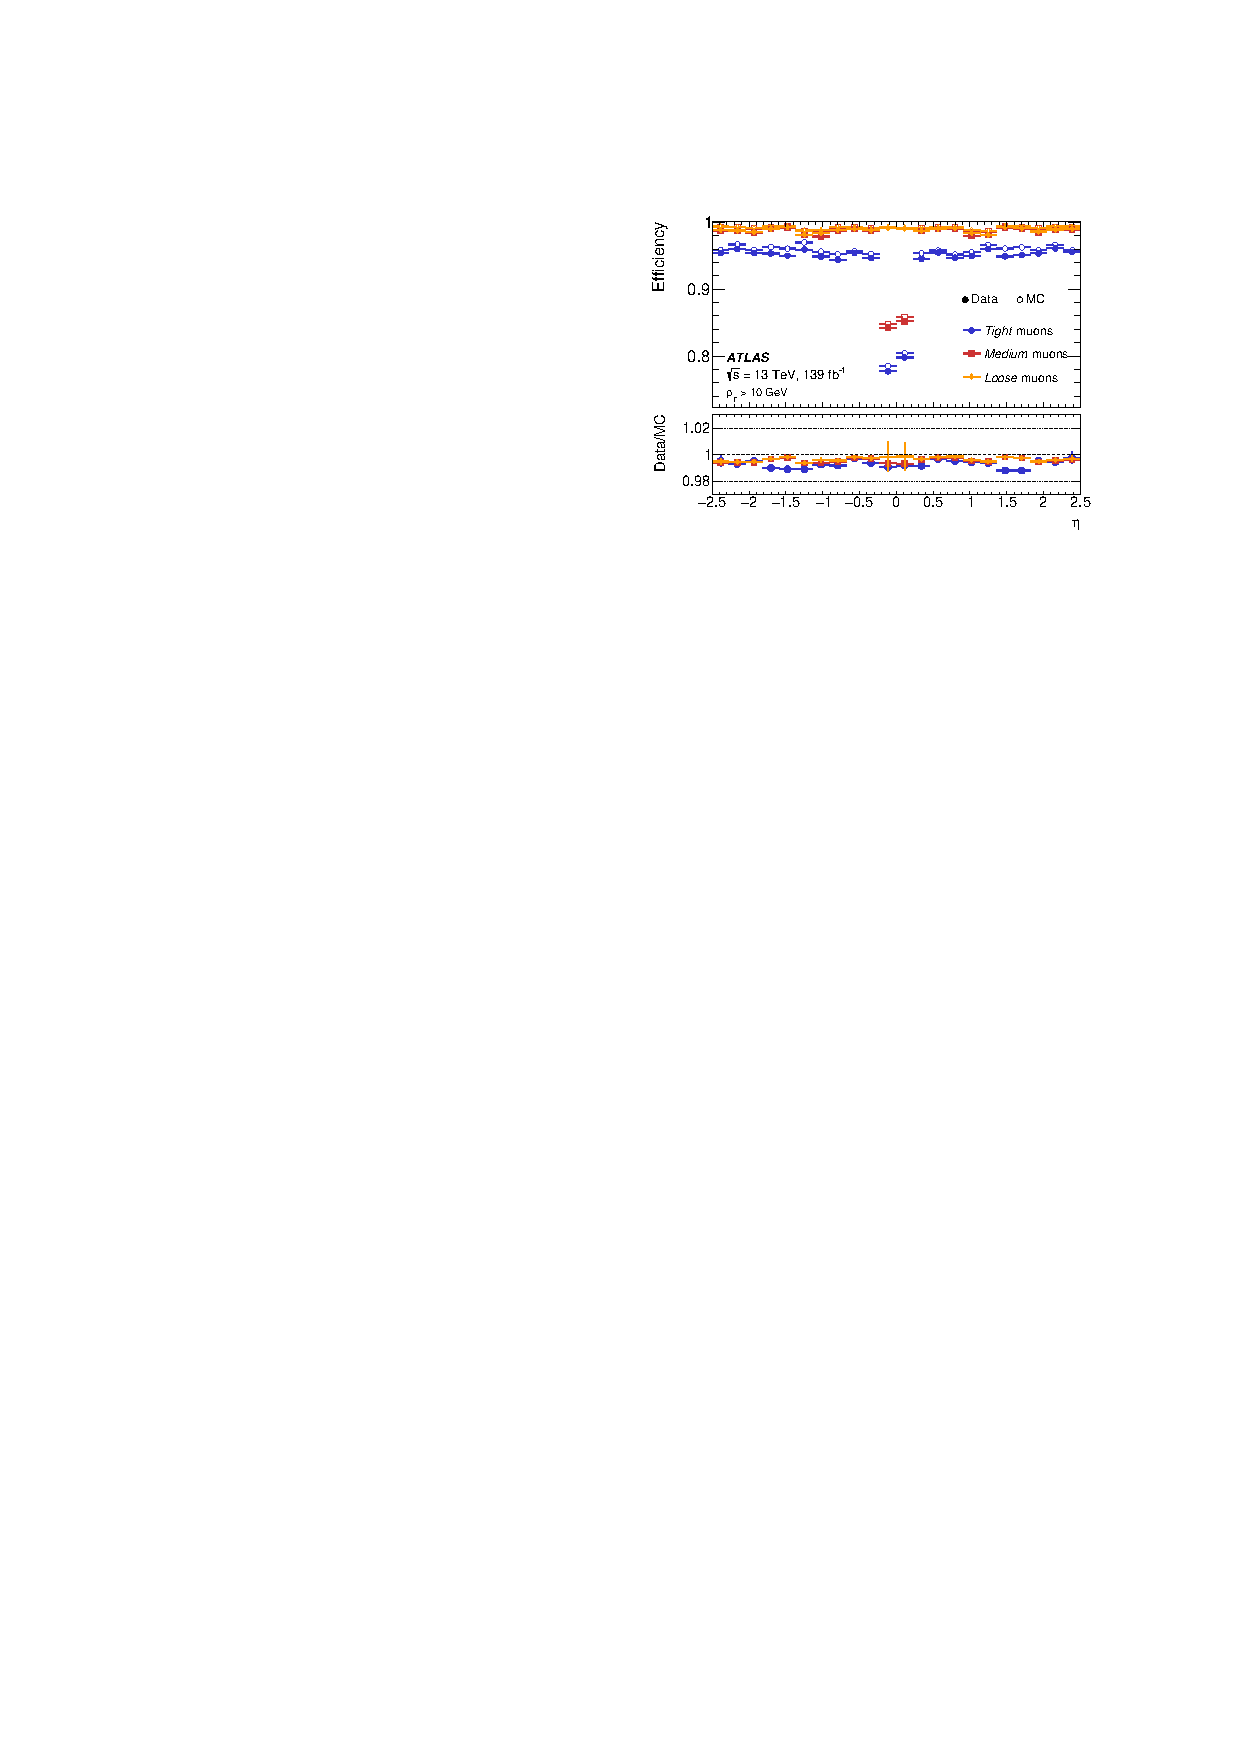
\includegraphics[width=0.49\textwidth]{images/muonIDeff_eta.pdf}
  }
  \hfill
  \subfloat[]{
      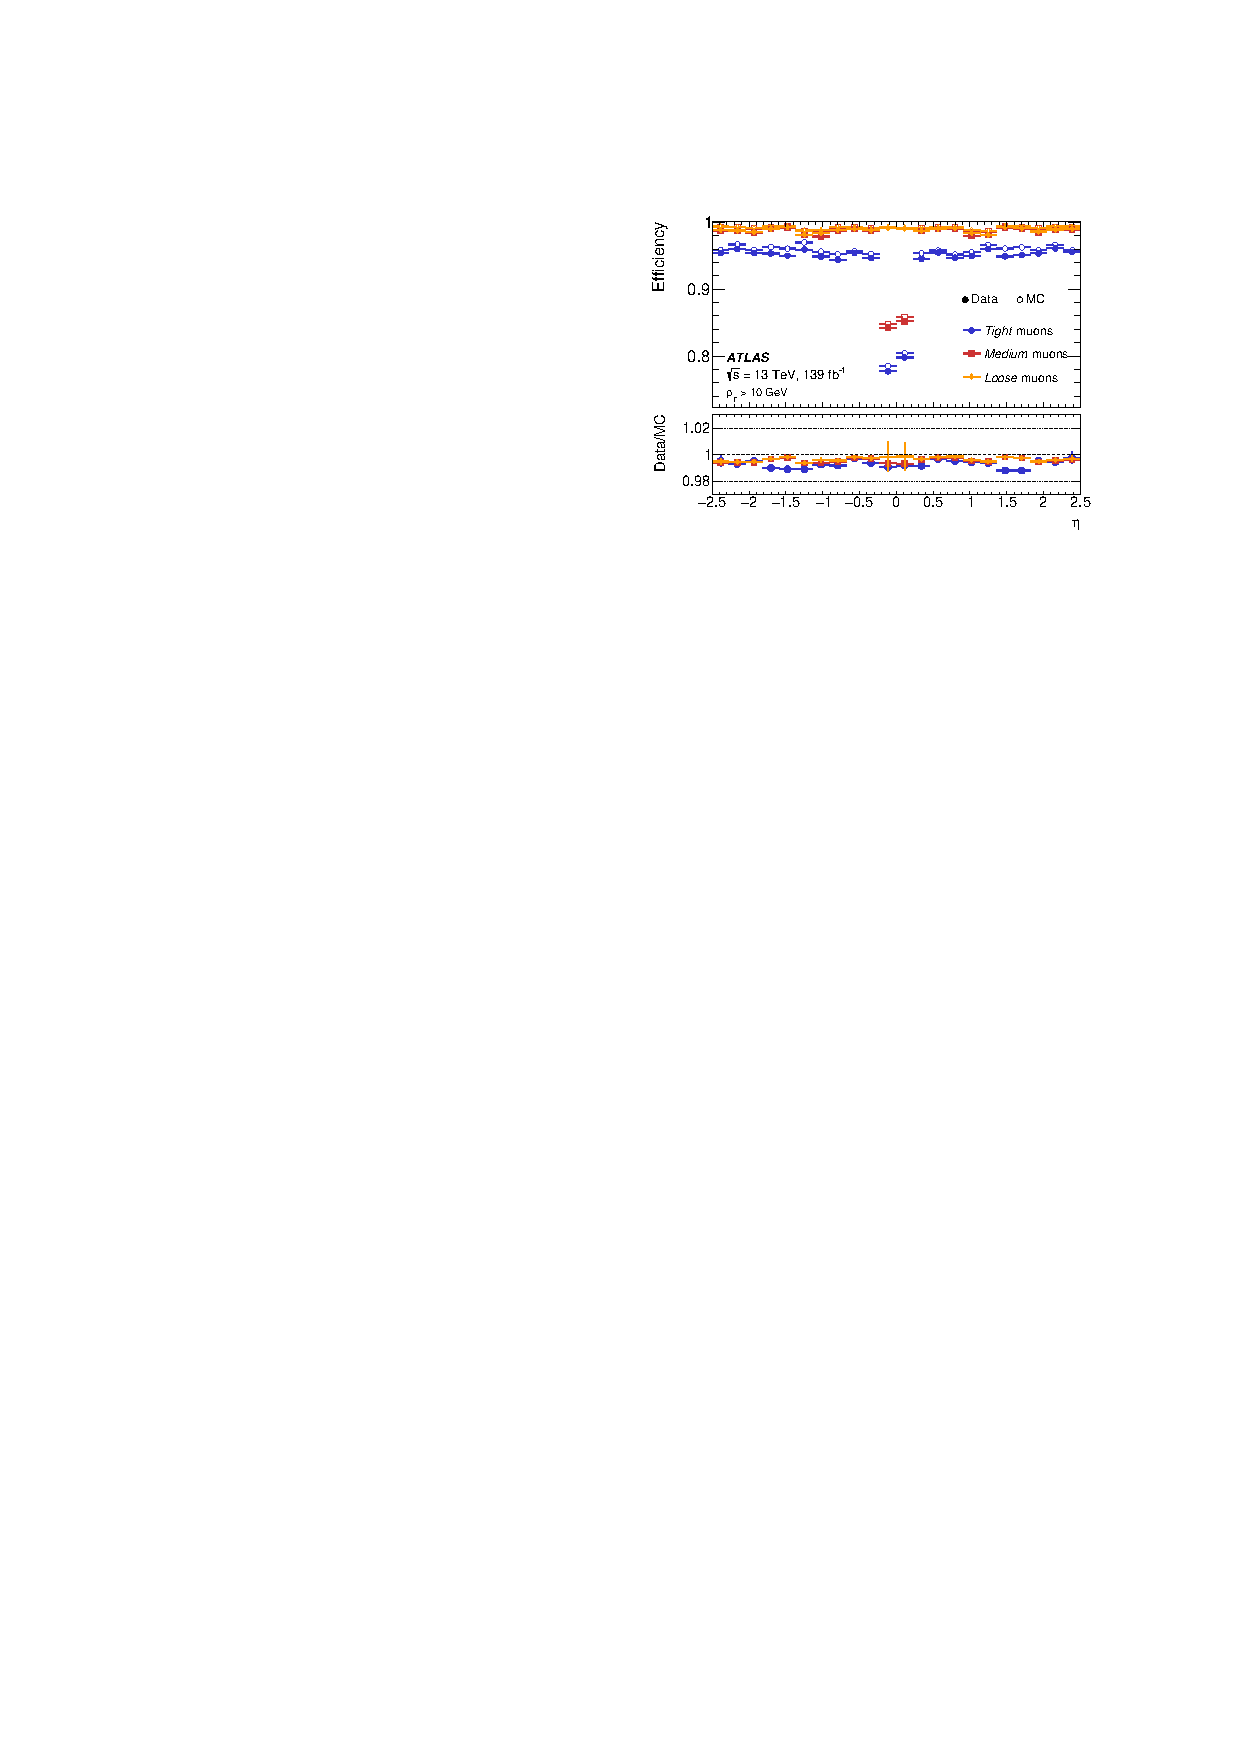
\includegraphics[width=0.49\textwidth]{images/muonIDeff_eta.pdf}
  }
  \caption{Muon reconstruction and identification efficiencies for the Loose, Medium, and Tight working points. Panel (a) shows efficiencies as a function of $p_{\text{T}}$ measured in $J/\psi \to \mu^+\mu^-$ events, and panel (b) shows efficiencies as a function of $\eta$ measured in $Z \to \mu^+\mu^-$ events with $p_{\text{T}}>10$~GeV. The lower panels display the data-to-MC scale factors with statistical and systematic uncertainties~\cite{muon_reco_run2}.}
  \label{fig:muon_eff}
\end{figure}

\subsection*{Isolation} 

Since prompt muons are typically produced without the presence of additional particles, muon isolation is applied to reject non-prompt candidates. Here, isolation quantifies additional detector activity around the muon, while the decay of high-momentum objects, whose products are often collimated, including muons, can naturally appear isolated.
Two isolation variables are used. Track-based isolation is defined as the scalar sum of the transverse momenta of all tracks with $p_{\text{T}}>1$~GeV within a cone around the muon (excluding the muon itself), where the cone size shrinks with increasing muon momentum, $p^{\mu}_{\text{T}}$, as $\Delta R = \text{min}(0.3, 10~\text{GeV}/p^{\mu}_{\text{T}})$.
Calorimeter-based isolation is computed by summing the energy deposits of topoclusters within a fixed cone of $\Delta R=0.3$ around the muon (again excluding the muon’s own deposit) and applying pile-up corrections. Each isolation criterion is then expressed as a ratio of the isolation sum to the muon’s transverse momentum.
Several working points are defined: Loose, Gradient, and FCTight (“fixed-cut tight”) all use both track- and calorimeter-based isolation; FCTO (“fixed-cut track-only”) applies only the track-based requirement.

\section{Jets and flavour tagging}
\label{sec:jets}
As explained in Section~\ref{subsec:proton}, in the proton-proton collisions the quarks and gluons produced at the partonic level undergo hadronisation, resulted in collimated jets measured by the ATLAS detector via the tracks registered in the ID and energy deposits in the calorimeter system. 

Jet reconstruction in ATLAS is fundamentally based on sequential recombination algorithms, the most widely used being the \antikt algorithm~\cite{Cacciari_2008}. This algorithm is designed to be stable in the presence of soft and collinear emissions from partons, operating by defining a distance measure between any two objects $i$ and $j$ (which may be tracks or topoclusters) as follows:
\begin{equation}
  d_{i,j} = \text{min}(p^{2p}_{\text{T},i},p^{2p}_{\text{T},j})\frac{\Delta^{2}_{ij}}{R^{2}},
\end{equation}
being $\Delta^{2}_{ij} = (\eta_{i} - \eta_{j})^2 + (\phi_{i} - \phi_{j})^2$ the distance in the $\eta$-$\phi$ plane and $R$ the radial parameter that defines the jet size. Setting the exponent $p=-1$ ensures that objects with higher transverse momenta dominate the clustering procedure. The beam distance is also computed for each object as:
\begin{equation}
  d_{iB} = p^{2p}_{\text{T},i},
\end{equation}
so the smaller of the two distance measures is chosen at each iteration. If $d_{ij}<d_{iB}$, objects \(i\) and \(j\) are merged into a new object. If $d_{iB}<d_{ij}$ then object \(i\) is identified as a jet and removed from the list of objects to process, and the procedure continues until no objects remain. The parameter \(R\) sets the jet radius and the extent of the \(\eta\)–\(\phi\) space used for clustering. It typically takes values of \(R = 0.4\) for small-radius jets or \(R = 1.0\) for large-radius jets~\cite{jets_cluster}.

Once jets are reconstructed, several energy calibrations are applied to correct for detector effects and achieve an accurate matching to the jet energy at particle level~\cite{jets_calib}. The first stage of jet calibration addresses pile-up effects arising from additional proton–proton interactions. An event-by-event correction is computed using the jet area and the transverse momentum density of the event, followed by residual corrections that depend on the number of reconstructed primary vertices and the average pile-up multiplicity. 

Next, the Jet Energy Scale (JES) calibration adjusts each jet reconstructed energy and pseudorapidity so that, on average, it matches the true particle-level jet energy. This is achieved via $p_{\text{T}}$- and $\eta$-dependent scale factors derived from full detector simulation, accounting for the differing calorimetric response to electromagnetic versus hadronic showers. After JES, a Global Sequential Calibration (GSC) applies multiplicative corrections based on the jet internal properties, such as width, track–vertex association, and flavor-sensitive observables, in order to reduce residual biases between quark- and gluon-initiated jets and to compensate for variations in fragmentation.

An in-situ calibration then removes any remaining mismodeling by comparing the balance between jets and well-measured reference objects (like isolated photons) in data; these data-driven correction factors, supplemented by multijet balance methods, are applied only to data jets to align their response with simulation. The Jet Energy Resolution (JER)~\cite{Aaboud_2017} is subsequently measured using dijet balance and random-cone techniques, yielding a $p_{\text{T}}$- and $\eta$-dependent resolution function. Simulation jets are smeared to reproduce the observed resolution in data.

Finally, to suppress pile-up jets, the Jet Vertex Tagger (JVT)~\cite{ATL-PHYS-PUB-2014-001} exploits track-based variables, particularly the fraction of jet tracks originating from the primary vertex, together with event-level pile-up information, to discriminate hard-scatter jets within $|\eta|<2.4$. For the forward region $(2.4<|\eta|<4.5)$, the forward JVT (fJVT) extends this technique, ensuring consistent pile-up rejection across the full calorimeter acceptance. 

\subsection*{Jet flavour tagging} 
Identifying jets originating from $b$-quarks (also referred to as $b$-jets) is vital for many LHC analyses, especially those involving top quarks or Higgs bosons. The $b$-hadrons travel a few millimeters before decaying, creating displaced secondary (and sometimes tertiary) vertices and tracks with large impact parameters relative to the primary collision point.
Simple $b$-taggers, like IP2D and IP3D, exploit these features by measuring the significance of transverse and longitudinal impact parameters and creating discriminants that recognizes tracks associated to non-primary vertex~\cite{btag_1,btag_2}, while secondary-vertex algorithms reconstruct displaced vertices and use features like invariant mass of tracks associated to the secondary vertex, vertex flight distance, and track multiplicity to distinguish $b$-jets from light-flavor or gluon jets.

Modern high-level $b$-taggers combine these low-level discriminants via machine learning techniques in order to improve the overall performance, also being able to tag intermediate $c$-hadrons and involved tertiary vertices. The DL1r algorithm, used for the first round of Run-2 data~\cite{tagging}, for example, feeds IP2D, IP3D, and secondary-vertex outputs into a deep neural network, along with additional variables, such as those from a jet-vertex finder, for improved $c$-jet rejection and an RNN to capture track correlations. DL1r produces three scores, corresponding to the probabilities that a jet originates from a $b$-, $c$-, or light quark, achieving superior separation compared to individual taggers.

The performance of $b$-tagging algorithms is characterized by the efficiency to identify $b$-jets and the rejection factors achieved against $c$-jets and light-flavor jets. Standard WPs are defined at approximately 60\%, 70\%, 77\%, and 85\% $b$-jet efficiency in \ttbar Monte Carlo events, trading off signal efficiency against background suppression.  To correct for residual differences between simulation and data, per-jet scale factors are measured in control regions with well-known flavor content (e.g.\ $t\bar t$ events) and applied to all Monte Carlo samples so that the simulated tagging efficiencies reproduce those observed in collision data.

For rel.22, the ATLAS $b$-tagging algorithm has evolved from the DL1r-based Deep Neural Network to the enhanced GN2 network~\cite{new_tagging}, which integrates Graph Neural Network techniques to better capture the relational information among tracks and secondary vertices. GN2 demonstrates improved separation power between \(b\), \(c\), and light-flavour jets, particularly at high pile-up, yielding a ~10\% gain in light-jet rejection at the 70\% \(b\)-jet efficiency WP compared to DL1r.  


\section{Hadronically decaying $\tau$-leptons}
\label{sec:tauhad}
Electrons and muons, usually referred to as light leptons, interact with the detector material and leave clear signatures. Due to their greater mass, \(\tau\)-leptons decay rapidly after approximately \(1\ \mu\mathrm{m}\), without reaching any detector layer. Therefore, they are reconstructed and identified from their decay products. The \(\tau\)-leptons can decay leptonically, to electrons or muons plus neutrinos (manifesting as missing transverse energy, \(E_{\mathrm{T}}^{\mathrm{miss}}\)), so no specialized reconstruction is performed in those cases. 
In fact, a key feature distinguishing these leptons from prompt leptons produced directly in the hard scattering is that the \(\tau\)-decay vertex is slightly displaced from the \(pp\) primary vertex. This is due to the finite lifetime of the \(\tau\)-lepton, resulting in an impact-parameter distribution for the final-state leptons that differs from that of prompt leptons. 
On the other hand, for hadronically decaying \(\tau\)-leptons (\(\tau_{\text{had}}\) from now on), which account for a total branching ratio of 65\%, a dedicated reconstruction and identification procedure exists, since these decays produce jets composed primarily of charged and neutral pions~\cite{PhysRevD.98.030001}.

The reconstruction of the visible products of hadronically decaying $\tau$-leptons ($\tau_{\text{had-vis}}$) begins with jets as seeds, clustered using the anti-\(k_{t}\) algorithm with a radius parameter \(R = 0.4\).  Candidates are required to satisfy \(p_{\text{T}} > 10\ \mathrm{GeV}\) and \(|\eta| < 2.5\).  The \(\tau\)-lepton energy is initially estimated by summing the energies of topoclusters within a cone of \(\Delta R = 0.2\) around the seed jet axis.  Within the same cone, the transverse momenta of all associated tracks are summed to reconstruct the \(\tau\)-lepton decay vertex.  
The vertex with the highest summed \(p_{\text{T}}\) is chosen, and only tracks with \(p_{\text{T}} > 1\ \mathrm{GeV}\), at least two pixel hits, and at least seven hits in the SCT and TRT are retained.  Impact-parameter requirements relative to the \(\tau\)-lepton vertex are \(|d_{0}| < 1.0\ \mathrm{mm}\) and \(|z_{0}\sin\theta| < 1.5\ \mathrm{mm}.\)
The \(n\)-prong \(\tau_{\text{had}}\) decay can consist of \(n\) charged hadrons (mostly pions, occasionally kaons), so candidates are categorized as 1-prong or 3-prong.  During rel.21, a dedicated Boosted Decision Tree (BDT) was trained to classify these track patterns; for rel.22, this was replaced by a Recurrent Neural Network (RNN) for \(\tau\)-lepton track classification~\cite{ATL-PHYS-PUB-2022-044}.  

After reconstructing the \(\tau_{\text{had-vis}}\) candidate, distinguishing it from quark- and gluon-initiated jets that can mimic its signature is achieved using separate RNNs for 1-prong and 3-prong \(\tau_{\text{had}}\) decays.  These networks are trained to be robust across the full \(p_{\text{T}}\) spectrum of the \(\tau_{\text{had-vis}}\) and under varying pile-up conditions, exploiting features of the \(\tau\)-lepton—namely its weak decay, which produces narrower jets with lower track multiplicities than QCD jets.  
The RNN output defines four working points (Tight, Medium, Loose, VeryLoose), with 1-prong efficiencies of 60\%, 75\%, 85\% and 95\%, and 3-prong efficiencies of 45\%, 60\%, 75\% and 95\%, respectively, balancing signal retention against background rejection.  For rel.22 this RNN has been superseded by a Graph Neural Network (similar to that used for \(b\)-tagging~\cite{new_tagging}), yielding significantly improved fake-\(\tau_{\text{had}}\) rejection and reducing this background by up to 40\% in our analysis.  

Finally, in rel.21, an additional BDT, known as the electron-veto BDT (eBDT), was trained to reject background from electrons that can mimic 1-prong \(\tau_{\text{had}}\) decays.  The eBDT uses high-level inputs such as calorimeter cell deposits and track features, with TRT information playing a crucial role in distinguishing electrons from hadrons.  It achieved over 95\% efficiency for genuine \(\tau_{\text{had}}\).  For rel.22, this task is now performed by a dedicated RNN~\cite{ATL-PHYS-PUB-2022-044}.

\section{Missing transverse momentum}
\label{sec:met}

Energy–momentum conservation guarantees that the total four–momentum of the initial state equals that of the final state.  In \(pp\) collisions, the longitudinal momentum cannot be determined because the colliding partons carry unknown fractions of the proton momentum.  However, since the incident protons travel and collide along the longitudinal axis, the total momentum in the transverse plane must be zero.  

Thus, the \etmiss quantifies the transverse energy carried away by invisible particles in the collision, as seen by the ATLAS detector.  These invisible particles may be neutrinos or other weakly interacting species such as dark matter candidates.  It is computed as the negative vector sum of all reconstructed and calibrated objects in ATLAS:

\begin{equation}
  \begin{split}
    \etmiss = \underbrace{- \sum_{\text{electrons}} p_{\text{T}}^{e} 
    + \sum_{\text{muons}} p_{\text{T}}^{\mu} 
    + \sum_{\text{photons}} p_{\text{T}}^{\gamma} 
    + \sum_{\text{taus}} p_{\text{T}}^{\tau} 
    + \sum_{\text{jets}} p_{\text{T}}^{j}}_{\text{hard term}}
    \underbrace{- \sum_{\text{unused tracks}} p_{\text{T}}^{\text{tracks}}}_{\text{soft term}}
  \end{split}
  \end{equation}
  

The missing transverse momentum has two contributions: the hard term, made up of calibrated electrons, photons, hadronically decaying \(\tau\)-leptons, jets, and muons, plus the soft term, which comprises energy not clustered into these objects. In ATLAS, the soft term is typically formed from tracks associated with the primary vertex, making it less sensitive to pile-up.

In simulations, the performance of \etmiss is validated by comparing MC and data in processes such as \(Z\to\mu^{+}\mu^{-}+\text{jets}\), where the true \etmiss is near zero.  Discrepancies can expose detector effects, jet miscalibration, or residual pile-up.  

    